\section{Business Model Canvas}
\label{sec:bmc}

Since we're creating a software product for people, there is a concern to make it viable for business too.
The tool we're using is Business Model Canvas.

Business Model Canvas\index{Business Model Canvas} (\ac{BMC})
is strategic management and lean startup template for developing new or documenting existing business models.
It is a visual chart with elements describing a firm's value proposition, infrastructure, customers, and finances.
It assists firms in aligning their activities by illustrating potential trade-offs.
% TODO

So with the Business Model Canvas, you can map out your entire business model in one image. This works for startup entrepreneurs, just as well as for the most senior executives.~\autocite{Strategyzer2011BMC}
Figure \autoref{fig:bmc:blank} shows how the blank Business Model Canvas looks like.

\begin{figure}[htbp]
    \centering
    %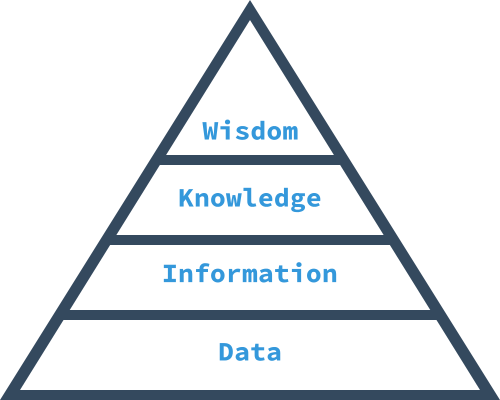
\includegraphics[width=4cm]{\dir/include/dikw-pyramid.png}
    \caption{Business Model Canvas}
    \label{fig:bmc:blank}
\end{figure}

For each building blocks...
%TODO


